\documentclass[xcolor=pdftex,dvipsnames,table]{beamer}
%\documentclass[xcolor=pdftex,dvipsnames,table,notes]{beamer} % slides + notes

% For more themes, color themes and font themes, see:
% http://deic.uab.es/~iblanes/beamer_gallery/index_by_theme.html
%
\mode<presentation>
{
  \usetheme{Warsaw}       % default, Darmstadt, Warsaw, Madrid ...
  \usecolortheme{orchid} % or try, orchid albatross, beaver, crane, default, ...
  \usefonttheme{serif}    % or try default, structurebold, ...
  
  \setbeamertemplate{headline}{}
  
  %gets rid of bottom navigation symbols
  \setbeamertemplate{navigation symbols}{}
  \setbeamertemplate{caption}[numbered]
  
  %\setbeamertemplate{footline}
  %{
 	%\leavevmode%
  	%\hbox{%
  	%\begin{beamercolorbox}[wd=.4\paperwidth,ht=2.25ex,dp=1ex,center]{author in head/foot}%
    %    \usebeamerfont{author in head/foot}\insertshortauthor
  	%\end{beamercolorbox}%
  	%\begin{beamercolorbox}[wd=.6\paperwidth,ht=2.25ex,dp=1ex,center]{title in head/foot}%
	%    \usebeamerfont{title in head/foot}\insertshorttitle\hspace*{3em}
	%    \insertframenumber{}/\inserttotalframenumber\hspace*{1ex}
  	%\end{beamercolorbox}}%
  	%\vskip0pt%
  %}
  
} 

%\setbeamertemplate{headline}{}

\usepackage[english]{babel}
\usepackage[utf8x]{inputenc}
\usepackage{chemfig}
\usepackage[version=3]{mhchem}
\usepackage{beamerthemesplit}
\usepackage{epigraph}
\usepackage{xcolor}
\usepackage{amsmath}
\usepackage{fixltx2e}
\usepackage{eso-pic}
\usepackage{framed, color}
\usepackage[framemethod=TikZ]{mdframed}
\usepackage{ragged2e}
\usepackage{caption}
\usepackage{graphicx}
\usepackage{subfig}
\usepackage{tcolorbox}

%\usetheme{Luebeck}

\mdfdefinestyle{MyFrame}{
    linecolor=blue,
    outerlinewidth=2pt,
    roundcorner=20pt,
    innertopmarn=\baselineskip,
    innerbottommargin=\baselineskip,
    innerrightmargin=20pt,
    innerleftmargin=20pt,
    backgroundcolor=gray!50!white
}

\graphicspath{{Images/}}

\author[Pérez D, Meneses E, Ropars T]{Diego Simón Pérez Arroyo}
%\date{\today}
\titlegraphic{
\includegraphics[scale=0.28]{logo.png}}

\institute{
	Thesis to opt for the degree of Magister Scientiae in Computing \\ 
    Supervisors: Esteban Meneses, Thomas Ropars
}
\title[Improving redundant multithreading  \hspace*{1em} \insertframenumber{}]{Improving redundant multithreading performance for soft-error detection in HPC applications}

\begin{document}

\begin{frame}
  \titlepage
\end{frame}

% ///////////////////////////////////////////////////////////////////////////////////////////////////////////////////////////
% ///////////////////////////////////////////////////////////////////////////////////////////////////////////////////////////
% ///////////////////////////////////////////////////////////////////////////////////////////////////////////////////////////
% ///////////////////////////////////////////////////////////////////////////////////////////////////////////////////////////

\section{Introduction}
\subsection{Problem Definition}

\begin{frame}
	\frametitle{Problem Definition}	   
    \only<1>{
		\begin{figure}[H]
    		\begin{center}
        		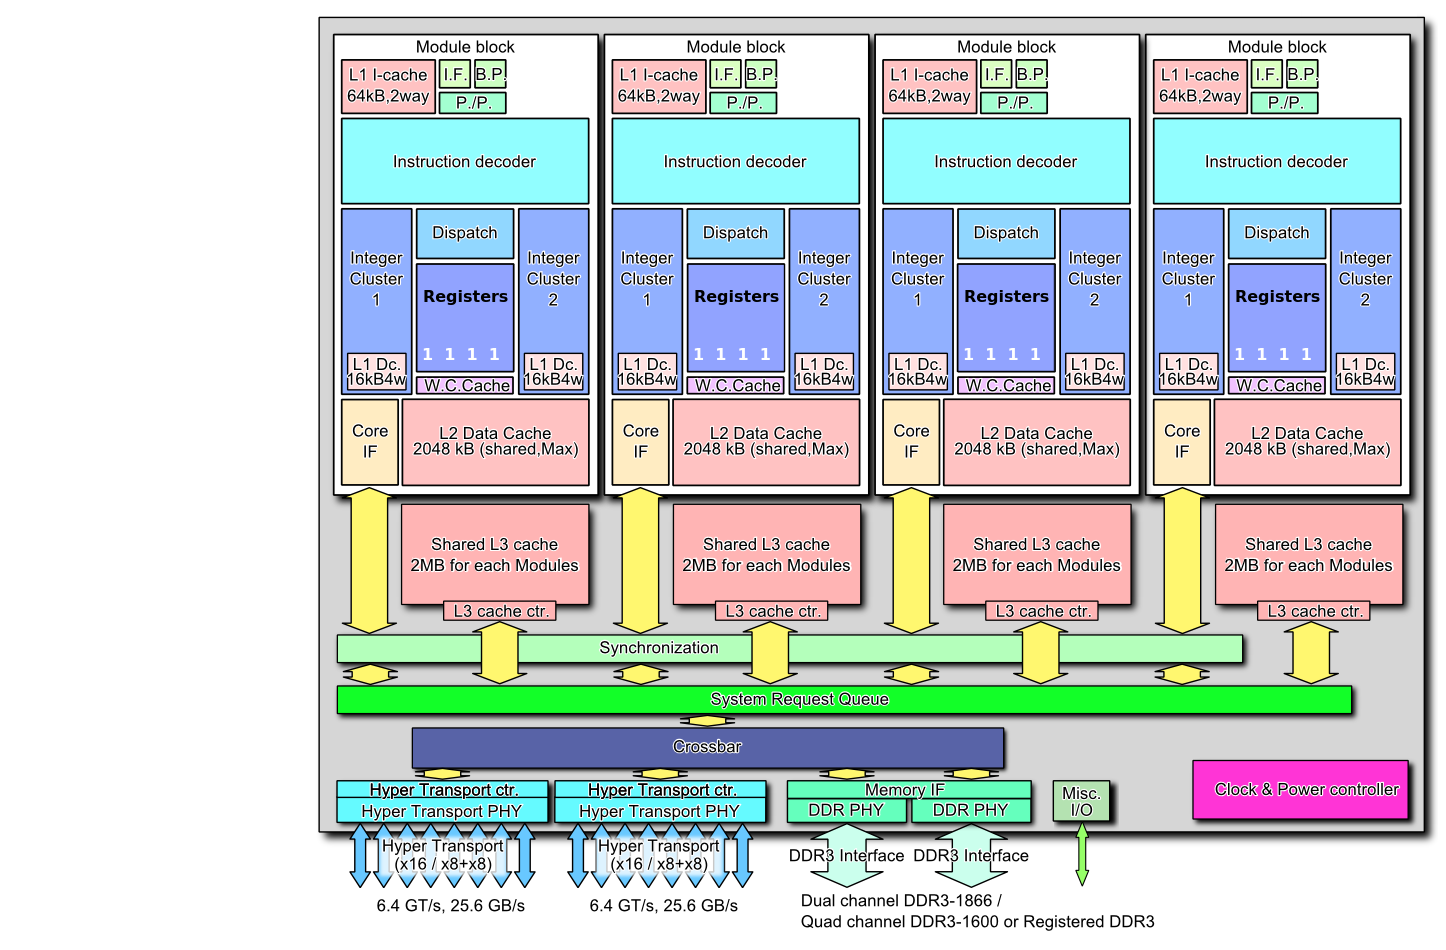
\includegraphics[scale=0.28]{Processor_Complexity-1.png}
    		\end{center}
   		\end{figure}
    }
    \only<2>{    	
        \begin{figure}[H]
    		\begin{center}
        		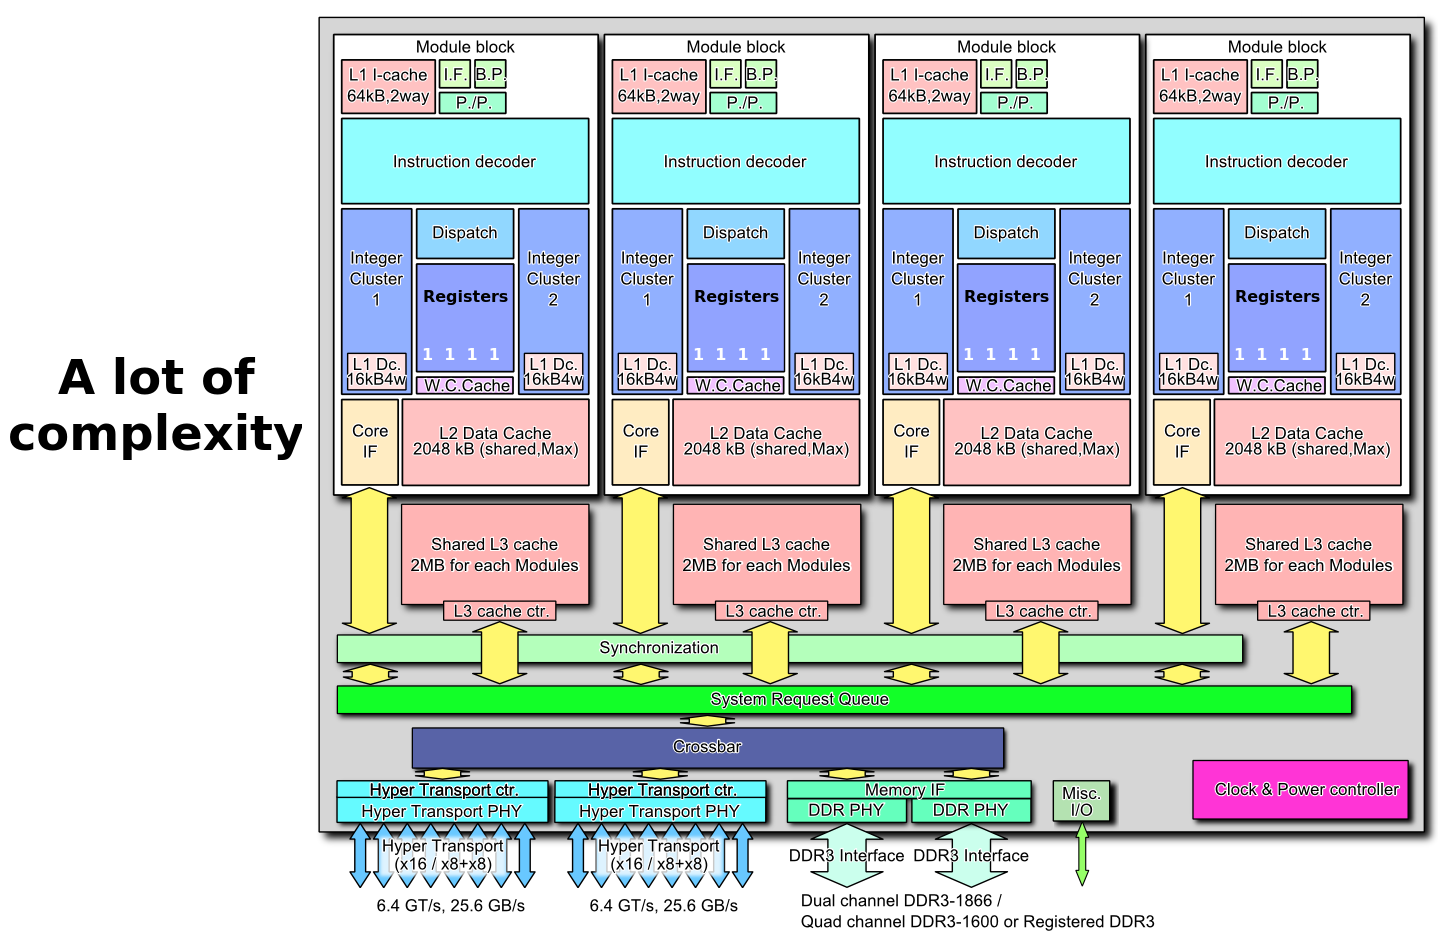
\includegraphics[scale=0.28]{Processor_Complexity-2.png}
    		\end{center}
   		\end{figure}
    }    
    \only<3>{
		\begin{figure}[H]
    		\begin{center}
        		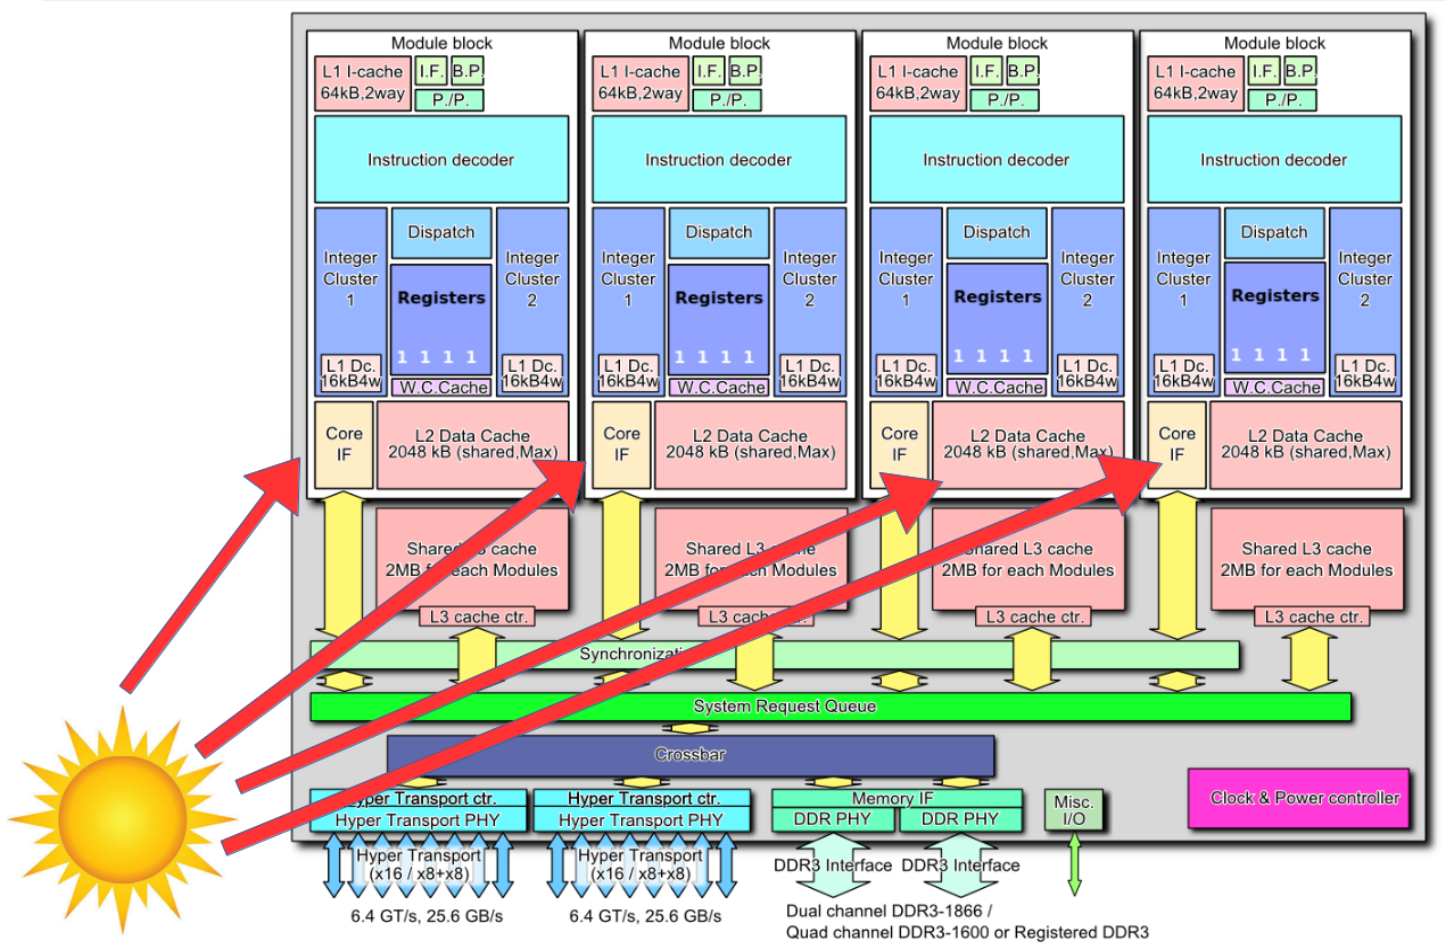
\includegraphics[scale=0.275]{Processor_Complexity-3.png}
    		\end{center}
   		\end{figure}
    }
    \onslide<4>{
		\begin{figure}[H]
    		\begin{center}
        		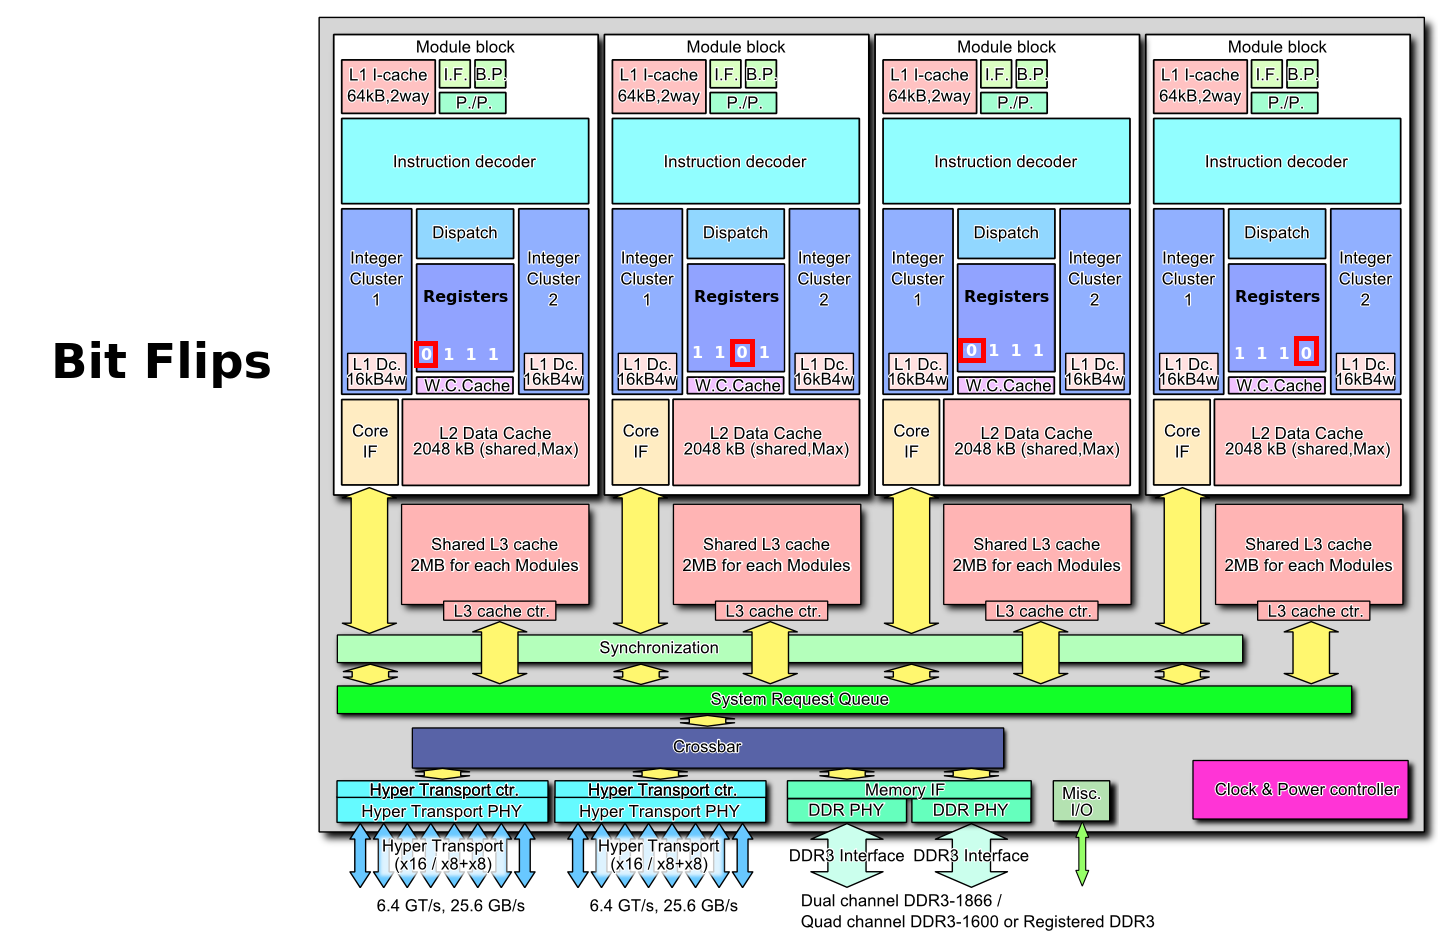
\includegraphics[scale=0.28]{Processor_Complexity-4.png}
    		\end{center}
   		\end{figure}
    }    
\end{frame}

\begin{frame}
	\frametitle{Problem Definition}		
	\begin{figure}[H]
    		\begin{center}
        		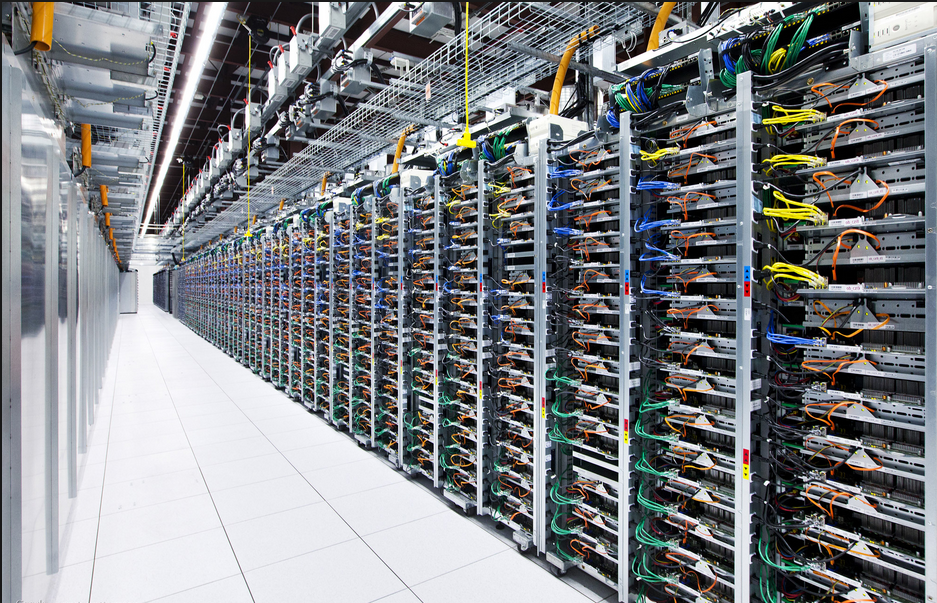
\includegraphics[scale=0.28]{DataCenter.png}
    		\end{center}
   		\end{figure}
\end{frame}


\begin{frame}
	\frametitle{Problem Definition - Redundant MultiThreading}		
	\begin{figure}[H]
    	\begin{center}
        	\captionsetup{labelformat=empty,labelsep=none}
        	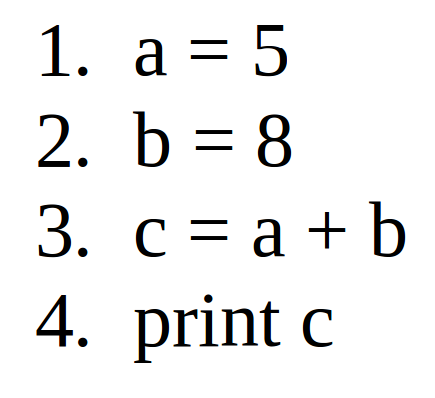
\includegraphics[scale=0.15]{OriginalCode.png}
            \caption{Original Code}
    	\end{center}
   	\end{figure}  
    
    \begin{figure}[H]
    	\begin{center}
            \captionsetup{labelformat=empty,labelsep=none}
        	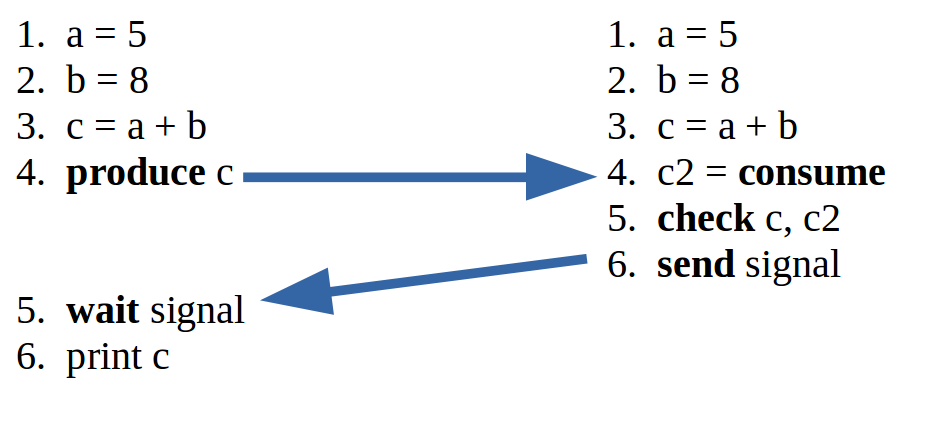
\includegraphics[scale=0.25]{RMT-Code.png}
            \caption{Redundant Multi-Threading Code}
    	\end{center}
   	\end{figure}  
\end{frame}


\begin{frame}
	\frametitle{Problem Definition - Redundant MultiThreading}	
	\begin{center}
		Inter-thread communication is a performance bottleneck.
	\end{center}    
	\begin{figure}[H]
    	\begin{center}
        	
\includegraphics[scale=0.35]{CommunicationCostMirror.jpg}
    	\end{center}
   	\end{figure}  
\end{frame}

%\begin{frame}
%	\frametitle{Problem Definition - Redundant Hyper-Threading}		
%	\begin{center}
%		Hyper-Threading helps because of shared L1 cache.
%	\end{center}    
	
%	\begin{figure}[H]
%    	\begin{center}
%        	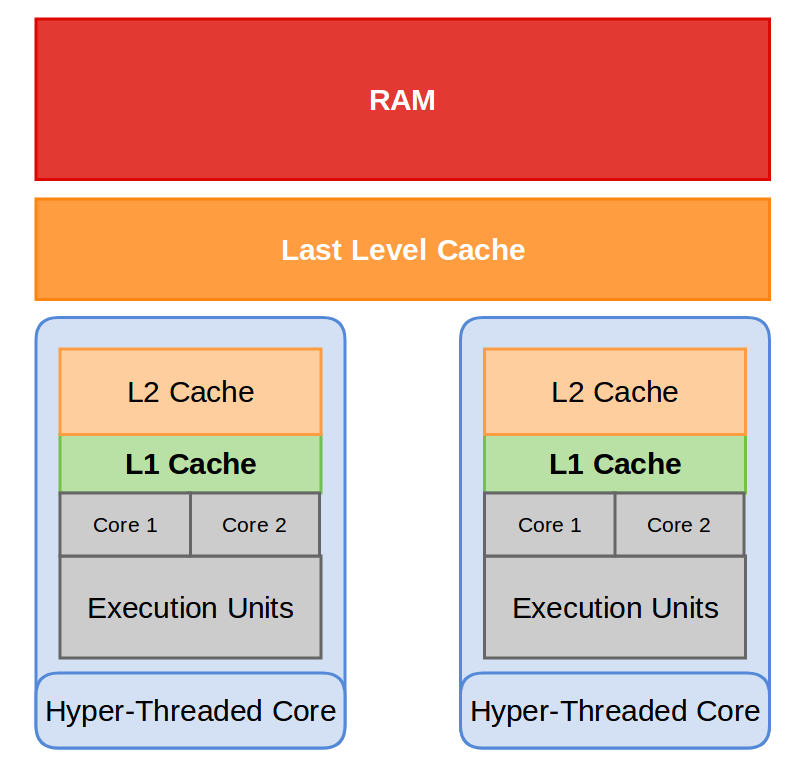
\includegraphics[scale=0.25]{HT-On-RMT.png}
%    	\end{center}
%   	\end{figure}  
%\end{frame}

\begin{frame}
	\frametitle{Thesis Proposal}		
	
	\begin{columns}[c]
		\column{2.3in}
		\begin{tcolorbox}[colback=blue!5,colframe=blue!40!black,title=Improve RMT performance]
            \begin{itemize}
        	    \item SMT to host sibling replicated threads on the same core.
        	    \item Variable aggregation, groups several values together.
        	    \item Selective checking, decreases the number of checked values to a minimum. 
            \end{itemize}
        \end{tcolorbox}
		
        \column{2in}
            \begin{figure}[H]
        	    \begin{center}
            	    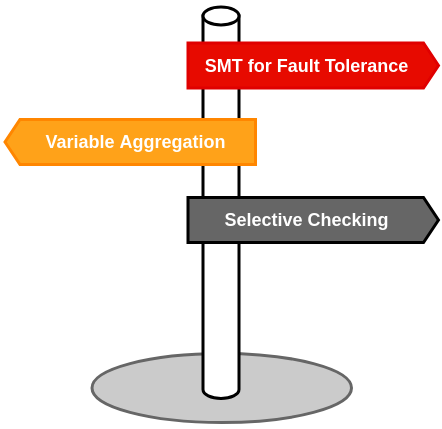
\includegraphics[scale=0.45]{3WaySign.png}
        	    \end{center}
       	    \end{figure}  
   	\end{columns}
	
\end{frame}

\begin{frame}
	\frametitle{Table of contents}
	\tableofcontents
\end{frame}

\subsection{Soft Errors: Causes and Consequences}
%\begin{frame}
%	\frametitle{The Soft Error Problem}

%	\begin{itemize}
%    	\item Complexity in multi-core processors (smaller transistors, energy reduction) places demands on fabrication quality. \pause
%        \item Several sources can invert the state of transistors and Silent Data Corruptions (SDC) may happen. \pause
%        \item Memory may be protected (ECC) but processor's registers are still vulnerable. 
%        \end{itemize}
        
        %\begin{figure}[H]
        %    \captionsetup{labelformat=empty,labelsep=none}
    	%	\begin{center}
        %    	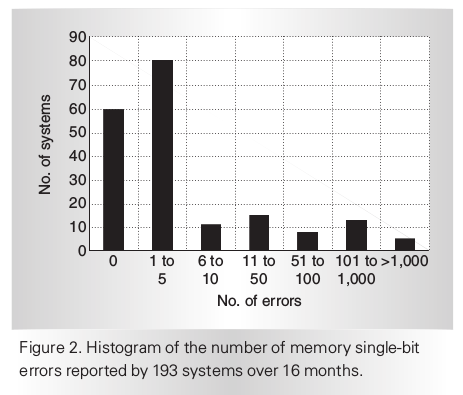
\includegraphics[scale = 0.3]{SoftErrorsHistogram.png}
        %        \caption{How often does it happens?}
        %    \end{center}
    	%\end{figure}
   	
%\end{frame}

\begin{frame}
	\frametitle{Soft Errors}
    \framesubtitle{Causes and Consequences}
	\begin{columns}[c]
		\column{2in}
          \onslide<1->{ \textbf{Causes}}
          \begin{itemize}
              \item \onslide<1->{ Cosmic radiation.}
              \item \onslide<1->{ Dynamic voltage scaling.}
              \item \onslide<1->{ Temperature, altitude.}
          \end{itemize}
        \column{2.5in}
          \onslide<2->{ \textbf{Consequences} }
          \begin{itemize}
              \onslide<2->{ \item Nothing, a bit flip in a unused address.}
              \onslide<2->{ \item Visible, segmentation fault, program hung.}
              \onslide<2->{ \item Silent, data corruption. }
          \end{itemize}
   	\end{columns}
	\onslide<1->{
    	\begin{figure}[H]
        	\captionsetup{labelformat=empty,labelsep=none}
    		\begin{center}
	    		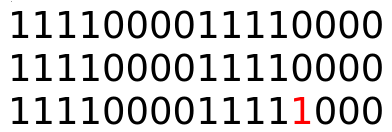
\includegraphics[scale=0.45]{SoftError.png}
            	\caption{A single bit flip}
    		\end{center}
    	\end{figure}  
    }
\end{frame}

%\note{
%	Un comentario sobre el slide, se apaga con la primer linea \\
%}

% ///////////////////////////////////////////////////////////////////////////////////////////////////////////////////////////
% ///////////////////////////////////////////////////////////////////////////////////////////////////////////////////////////
% ///////////////////////////////////////////////////////////////////////////////////////////////////////////////////////////
% ///////////////////////////////////////////////////////////////////////////////////////////////////////////////////////////

%\section{Soft Error Management}

%\subsection{Soft Error Correction}

%\begin{frame}
%	\frametitle{Soft Error Management}
%    \centerline{\textbf{Checkpointing}}
    
%    \begin{columns}[c]
%		\column{2in}
%        	\begin{figure}[H]
%        		\captionsetup{labelformat=empty,labelsep=none}
%   				\begin{center}
%					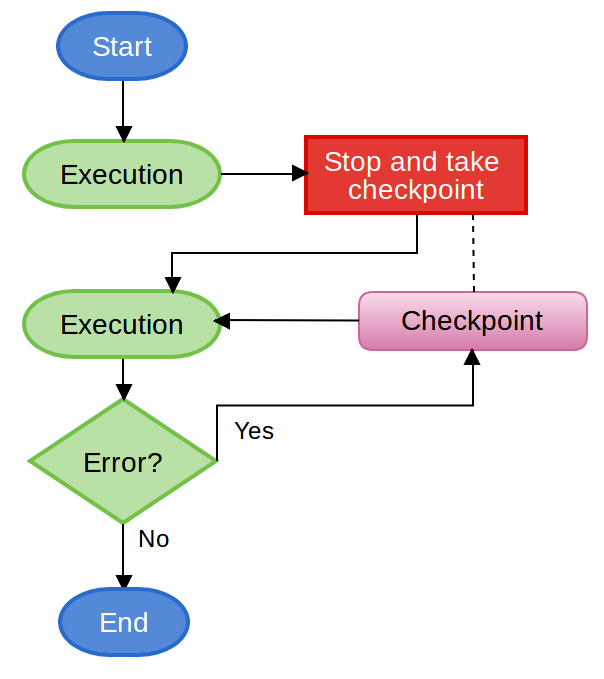
\includegraphics[scale=0.22]{Checkpointing.png} 
%    			\end{center}
%    		\end{figure}
        
%        \column{2.6in}
%        	\begin{itemize}
%    			\item Every certain amount of time (or instructions) the application's state is saved.
%        		\item If an error is found, the app is restored to last checkpoint. \pause
%                \item Penalty cost of stopping execution to create a checkpoint.
%                \item Is the commonly suggested option. 
%            \end{itemize}
            
%    \end{columns}
              
%\end{frame}

%\begin{frame}
%   \frametitle{Soft Error Management}
   	
%    \centerline{\textbf{Triple Modular Redundancy}}
    
%    \begin{itemize}
%    	\item 2 extra copies of the instructions. 
%        \item A majority vote is used each time to decide the correct result. 
        
%        \begin{figure}[H]
%    		\captionsetup{labelformat=empty,labelsep=none}
%    		\begin{center}
%        		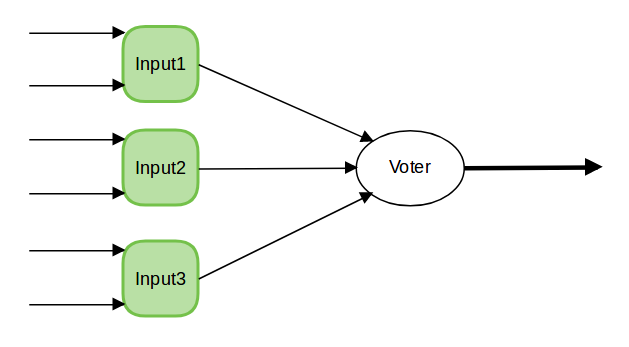
\includegraphics[scale=0.35]{TripleModularRedundancy.png} \pause
%        	\end{center}
%   		\end{figure} 
        
%        \item If an error is found, the mismatching copy can be disregarded. 
%        \item Significant performance overhead. 
%    \end{itemize}
              
%\end{frame}

\section{Soft Error Detection}

\begin{frame}
	\frametitle{Soft Errors Detection}        
    \definecolor{shadecolor}{rgb}{0.9,0.5,0.007}
    \begin{shaded}
    	\centerline{Redundancy: an operation is replicated and results are compared.}
        \centerline{If results are different $\Longrightarrow$ a soft error is detected.}\pause
    \end{shaded}      
    
	\begin{columns}[c]
		\column{2.4in}
          \textbf{Hardware Replication}
          \begin{itemize}
              \item Specialized hardware is in charge of replication. 
              \item Transparent to the programmer. 
              \item More chip size, more logic, more expensive (\$\$\$). \pause
          \end{itemize}
		\column{2.4in}
          \textbf{Software Replication}
          \begin{itemize}
              \item Requires programmer's intervention. 
              \item There is a non-negligible performance overhead.
              \item Common hardware is used, cheaper (\$).
          \end{itemize}
    \end{columns}
    
	%\definecolor{shadecolor}{rgb}{0.95,0.9,0.9}
    \definecolor{shadecolor}{rgb}{1,1,1} 
    \begin{shaded}
    	\centerline{}
    \end{shaded}
\end{frame}

\subsection{Software Replication}

\begin{frame}
	\frametitle{Software Replication - Instruction Level Redundancy}
    
    \begin{itemize}
    	\item Thread-local, everything happens on the main thread.  
        %\item Instruction are replicated (a shadow dataflow), frequent checks are also added.
        %\item Shadow dataflow uses different registers, which allows safe value comparisons.
        \item Checks happen in \textit{critical path}, which adds a lot of overhead. 
    \end{itemize}
    
          \begin{figure}[H]
            \begin{center}
                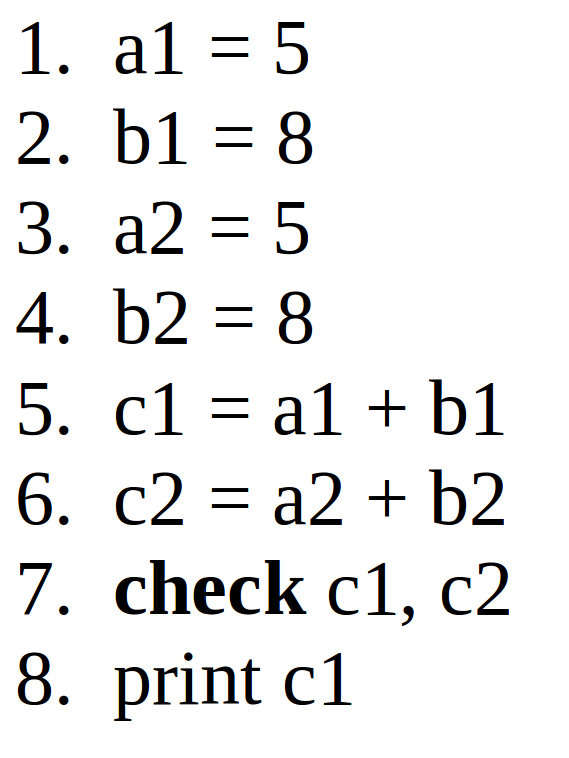
\includegraphics[scale=0.2]{ILR-Code.png}
            \end{center}
        \end{figure}
    
\end{frame}

\begin{frame}
	\frametitle{Software Replication - Redundant Multi-Threading}

	\begin{itemize}
    	\item Replication is distributed in two threads, leading or producer and trailing or consumer.
        \item Frequent inter-thread communication (performance bottleneck) is done via a SPSC queue. 
    \end{itemize}
    
    \begin{figure}[H]
    	\begin{center}
        	\captionsetup{labelformat=empty,labelsep=none}
        	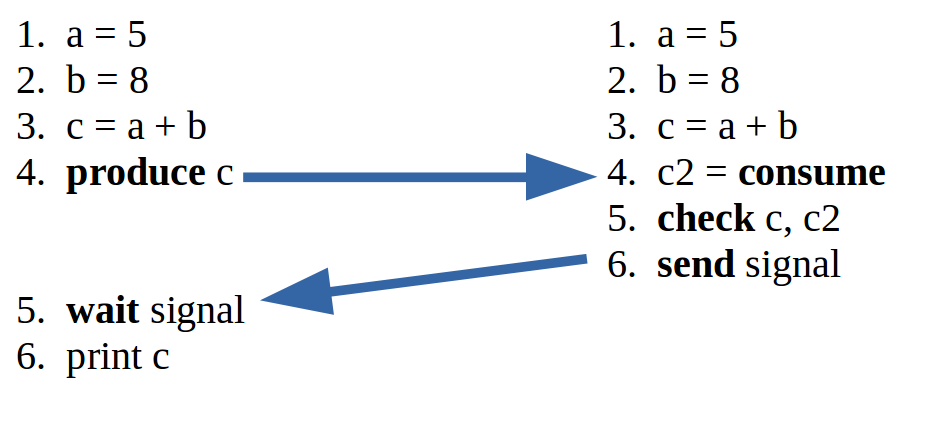
\includegraphics[scale=0.25]{RMT-Code.png}
            \caption{Redundant Multi-Threading Code}
         \end{center}
     \end{figure}
    
\end{frame}

\subsection{Redundant Multi-Threading}
\begin{frame}
	\frametitle{Redundant Multi-threading (RMT)}
    
    \definecolor{shadecolor}{rgb}{0.9,0.5,0.007}
    \begin{shaded}
    	\centerline{\textbf{Not all instructions are replicated}}
    \end{shaded}      
    \only<1>{
        \begin{figure}[H] 
        \captionsetup{labelformat=empty,labelsep=none}
            \begin{center}
                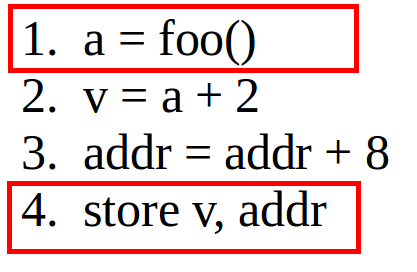
\includegraphics[scale=0.45]{OriginalCode2-2.png}
            \end{center}
        \end{figure}
    }\pause
    
    \only<2>{
        \begin{figure}[H]
        	\captionsetup{labelformat=empty,labelsep=none}
            \begin{center}
                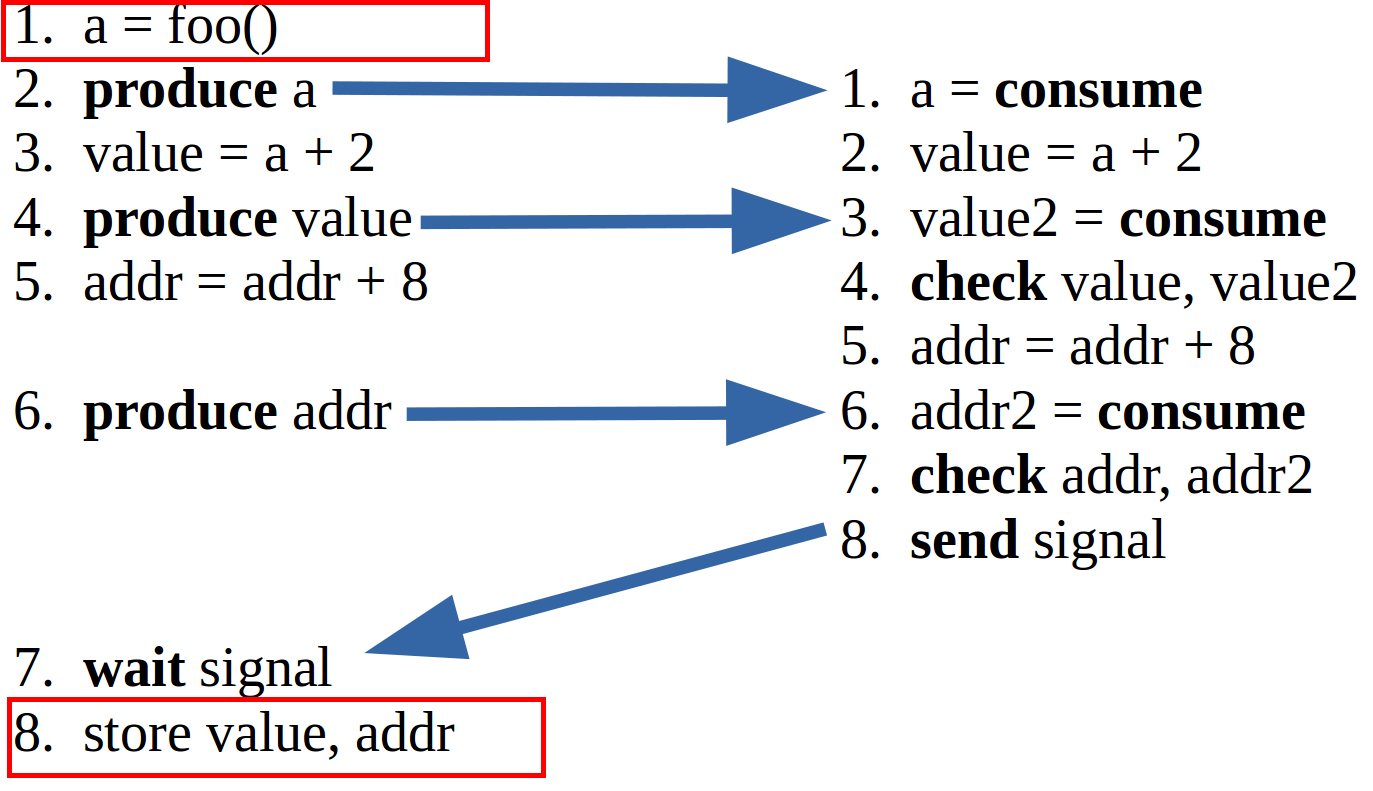
\includegraphics[scale=0.20]{RMT-Code-2-2.png}
            \end{center}
        \end{figure}
    }
    
    \textbf{Excluded: }
    \begin{itemize}
    	\item Library function calls.
    	\item Memory store/loads.
    \end{itemize}
\end{frame}

\begin{frame}
	\frametitle{RMT - Volatile Memory Accesses}
    
    \begin{itemize}      		   
   		\item A volatile variable is one that may be modified in ways unknown to the implementation.
        \item Memory-mapped IO accesses: network operations. \pause
        \item Wrong execution can be catastrophic and irreversible. 
    \end{itemize}
		
    \begin{figure}[H]
    	\begin{center} 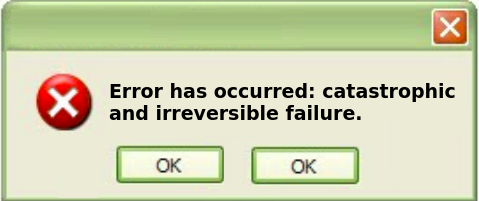
\includegraphics[scale=0.35]{CatastrophicFailure.png} \end{center} 
    \end{figure} \pause
   
     \underline{Multiple communication patterns}
        \begin{itemize}
    		\item Synchronous.
        	\item Asynchronous.
            \item Semi-synchronous.
    	\end{itemize}
    
\end{frame}

\begin{frame}
	\frametitle{RMT - Synchronous Communication Pattern}  
    
	\begin{columns}[c]
		\column{2in}
         	\begin{figure}[H]
            	\captionsetup{labelformat=empty,labelsep=none}
         		\begin{center} 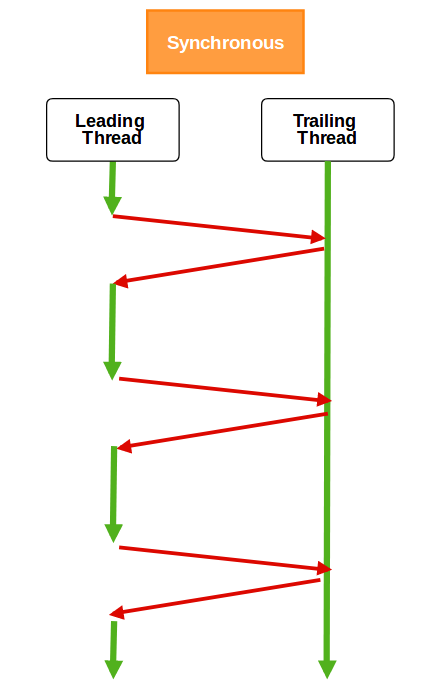
\includegraphics[scale=0.27]{Pattern-Sync.png} \end{center}
                Leading thread \textbf{waits} every time check from trailing thread. 
     		\end{figure}
            
		\column{3in}        
        	\begin{figure}[H]
        		\begin{center}
        			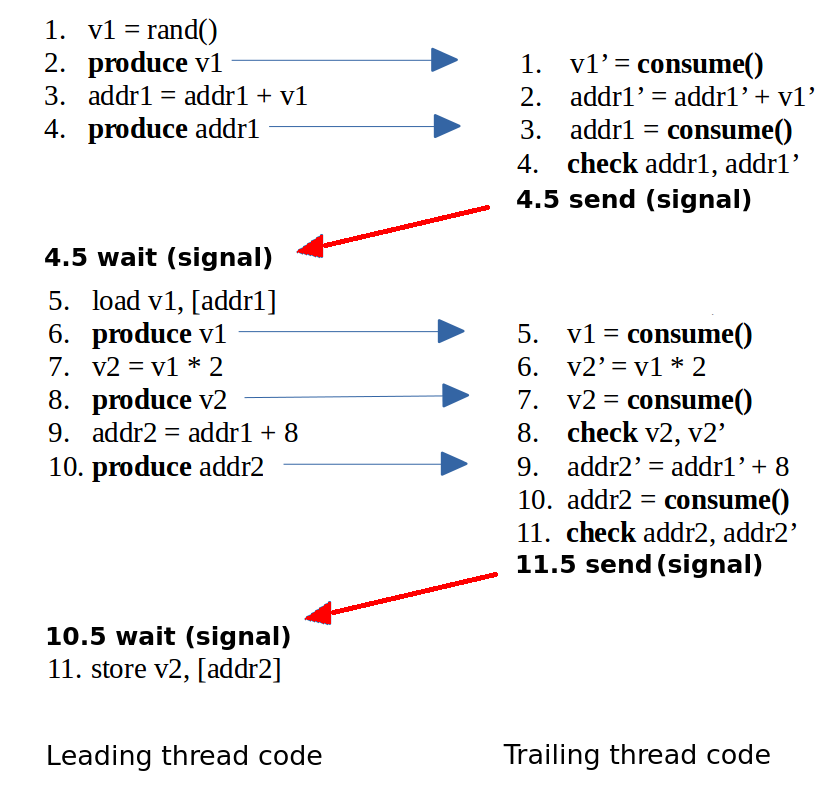
\includegraphics[scale=0.3]{CodeTransformation-Cyclic.png}
         		\end{center}
        	\end{figure}
            
    \end{columns} \pause
    
    \definecolor{shadecolor}{rgb}{0.9,0.5,0.007}
    \begin{shaded} \centerline{Safest but slowest.} \end{shaded}
                
    %\begin{itemize}
    	%\item Leading thread waits every time check from trailing thread. 
        %\item No problem with volatile stores. 
        %\item A lot of overhead.
    %\end{itemize}
        
\end{frame}

\begin{frame}
	\frametitle{RMT - Asynchronous Communication Pattern}  
    
	\begin{columns}[c]
		\column{2in}
         	\begin{figure}[H]
            	\captionsetup{labelformat=empty,labelsep=none}
         		\begin{center} 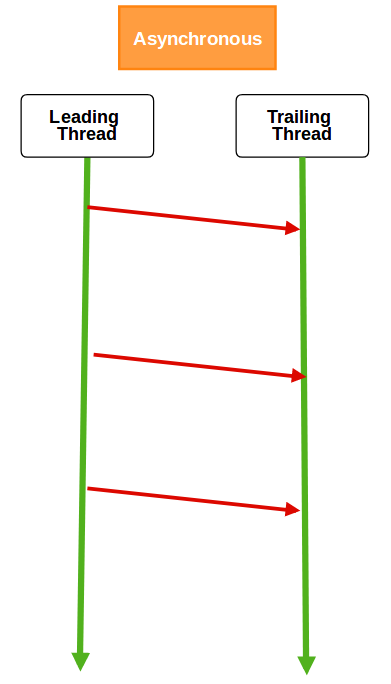
\includegraphics[scale=0.27]{Pattern-Async.png} \end{center}
                Leading thread \textbf{continues} without check from trailing thread.
     		\end{figure}
            
		\column{3in}        
        	\begin{figure}[H]
        		\begin{center}
                	\captionsetup{labelformat=empty,labelsep=none}
                	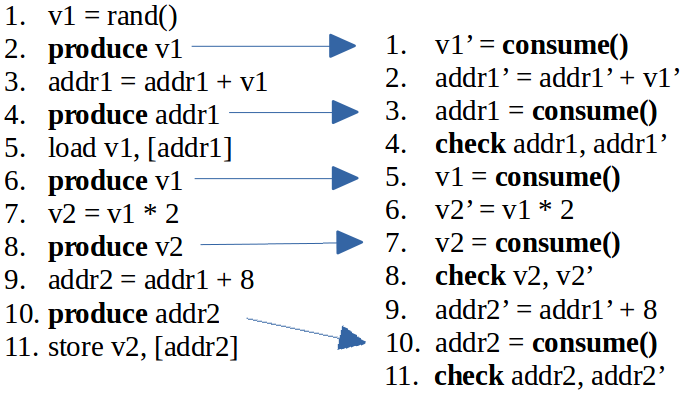
\includegraphics[scale=0.4]{CodeTransformation-NotCyclic.png}
                	\caption{Leading and trailing thread.}
                \end{center}
        	\end{figure}
            
    \end{columns} \pause
    
    \definecolor{shadecolor}{rgb}{0.9,0.5,0.007}
    	\begin{shaded}
    		\centerline{Fastest but insecure on volatile stores.}
    	\end{shaded}
                
    %\begin{itemize}
    %	\item Leading thread continues without check from trailing thread. \pause
    %   \item Error are later detected by the trailing thread. \pause
    %   \item Works fine as long as operations in the leading thread don't include volatile variable accesses. \pause
	%\end{itemize}
        
\end{frame}


\begin{frame}
	\frametitle{RMT - Semi-Synchronous Communication Pattern}  
    
	\begin{columns}[c]
		\column{2in}
         	\begin{figure}[H]
            	\captionsetup{labelformat=empty,labelsep=none}
         		\begin{center} 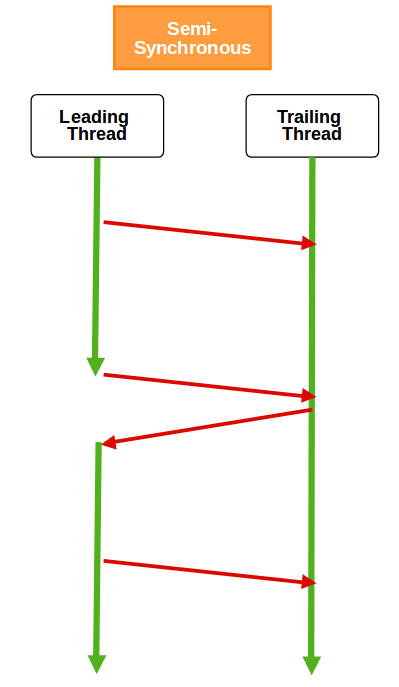
\includegraphics[scale=0.27]{Pattern-SemiSync.png} \end{center}
                Leading thread continues \textbf{as much as possible} without checks. 
     		\end{figure}
            
		\column{3in}        
        	\begin{figure}[H]
        		\begin{center}
                	\captionsetup{labelformat=empty,labelsep=none}
                	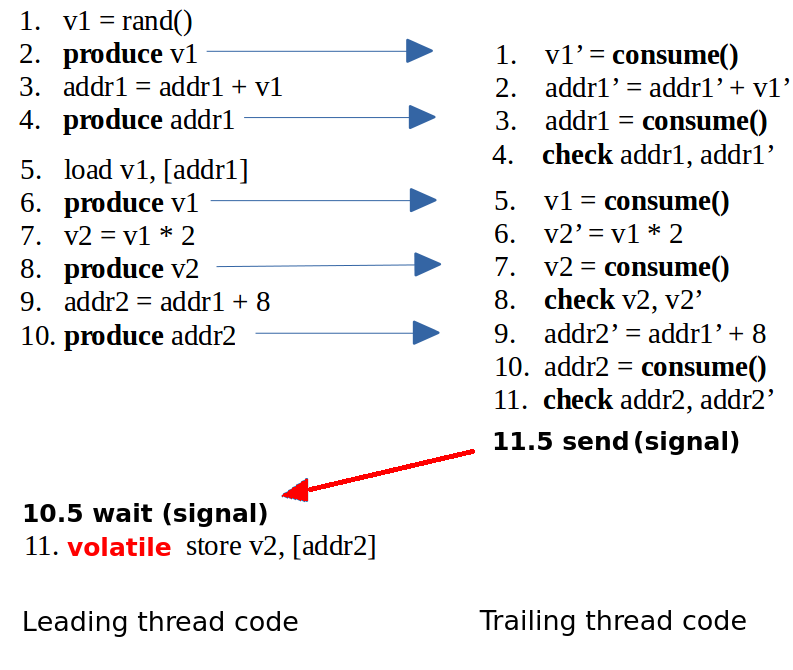
\includegraphics[scale=0.3]{Semi-Sync-CommunicationSyncing.png} 
                	\caption{Leading and trailing thread.}
                \end{center}
        	\end{figure}
            
    \end{columns} \pause
    
    \definecolor{shadecolor}{rgb}{0.9,0.5,0.007}
   	\begin{shaded}
    	\centerline{Preferred one, safe and fast.} 
    \end{shaded}
          
	%\begin{itemize}
    %          \item Leading thread continues as much as possible without checks. 
    %          \item Ensures correctness on volatile stores via ILR or syncing with the trailing thread. 
    %          \item Reduces communication overhead, while trailing thread still checks everything else. 
    %      \end{itemize}          
                  
\end{frame}
   
\begin{frame}
	\frametitle{Redundant Multi-Threading - Current Solutions}
        
   \emph{C. WANG, H. KIM, Y. WU,  V. YING, \textbf{Compiler-managed software-based redundant multi-threading for transient fault detection}, in Proceedings of the International Symposium on Code Generation and Optimization, IEEE, (2007).}
              
	\vskip 0.2in 
              
	\begin{itemize}
    	\item RMT with semi-synchronous communication pattern. 
        \item Few percentage of volatile variables does not affect performance much. 
        %\item Identify volatile variables with information available at compile time. \pause
    \end{itemize}
    
    \definecolor{shadecolor}{rgb}{0.9,0.5,0.007}
   	\begin{shaded}
    	\centerline{Our solution will use a similar approach.} 
    \end{shaded}
     
\end{frame}
   
   
\begin{frame}
	\frametitle{Redundant Multi-Threading - Current Solutions}  
    
    \emph{Y. ZHANG, J. W. LEE, N.P. JOHNSON, D. I. AUGUST, \textbf{Daft: decoupled acyclic fault tolerance}, International Journal of Parallel Programming, 40 (2012).}
    
    \begin{columns}[c]
    	\column{2.6in}
        	\begin{figure}[H]
            	\begin{center}
                	\captionsetup{labelformat=empty,labelsep=none}
                  	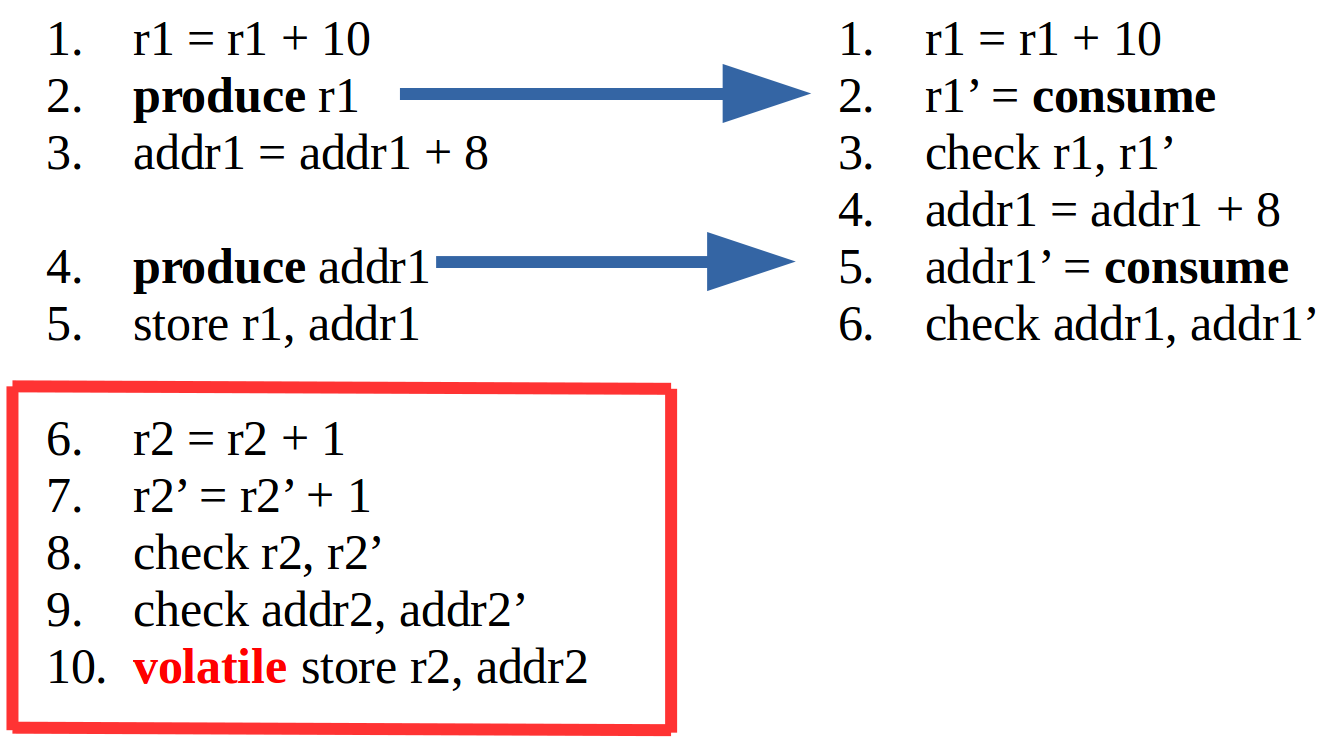
\includegraphics[scale=0.2]{Daft-Reduced.png} 
                  	\caption{Leading and trailing thread.}
              	\end{center}
          	\end{figure}
        \column{2in}
    	\begin{itemize}    
    		\item ILR for volatile memory accesses. \pause
            \item What about data dependencies? \pause
    	\end{itemize}	    		
        \definecolor{shadecolor}{rgb}{0.9,0.5,0.007}
   			\begin{shaded}
    			\centerline{+ data dependencies $\Rightarrow$ - RMT. } 
          \end{shaded}
    \end{columns}            
\end{frame}


\begin{frame}
	\frametitle{Intel Hyper-Threading (HT) - Benefit for RMT}
    \begin{columns}[c]
		\column{2in}
           \begin{figure}[H]
    			\begin{center}
                	\captionsetup{labelformat=empty,labelsep=none}
	    			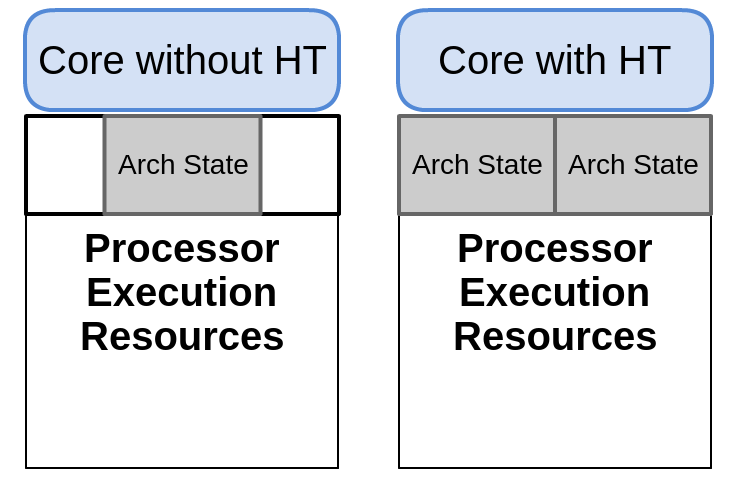
\includegraphics[scale=0.22]{HyperThreading.png}
            		\caption{Core with and without HT}
    			\end{center}
    	   \end{figure}
        \column{2.5in}
          \begin{itemize}
              \item Single physical processor appears as two logical processors. \pause
              \item Architecture state is duplicated. \pause
              \item Physical execution resources are shared: execution units, L1 cache. \pause  
              \item When one logical processor is stalled the other one could make forward progress.
          \end{itemize}
   	\end{columns}
\end{frame}

\begin{frame}
	\frametitle{Intel Hyper-Threading - Benefit for RMT}
    
    \definecolor{shadecolor}{rgb}{0.9,0.5,0.007}
    \begin{shaded}
    	\centerline{\textbf{How can Hyper-Threading benefit RMT?}}
    \end{shaded}
    
   \centerline{Intel Broadwell Xeon E5-2699v4 (2.2 GHZ) \footnote{https://www.anandtech.com/show/11544/intel-skylake-ep-vs-amd-epyc-7000-cpu-battle-of-the-decade/13}}
   
\begin{center}
    \begin{tabular}{| l | l | l |} \hline
    	\textbf{Memory Hierarchy} & \textbf{Clock Cycles }& \textbf{Nanoseconds} \\ \hline
    	RAM & 209 & 95 \\ \hline
    	Cache L3 & 38-51 & 17.27 - 23.18 \\ \hline
    	Cache L2 & 12-15 & 5.45 - 6.81 \\ \hline
    	Cache L1 & 4 & 1.81 \\ \hline    
    \end{tabular}
\end{center}   \pause
    
    \begin{itemize}     	    	
        \item Hyper-threads run on a single core, 50\% less resource overhead compared to threads on different cores.
    \end{itemize}
\end{frame}

\section{Research Proposal}
\subsection{Justification}
\begin{frame}
	\frametitle{Research Justification}
    
    \definecolor{shadecolor}{rgb}{0.9,0.5,0.007}
    \begin{shaded}
    	\centerline{HT in RMT has not been properly investigated.}
    \end{shaded}
    
    \begin{itemize}
        \item Tested only on 1 experiment (2007), finished second.
        \item Improvements of HT in the last 10 years? \pause
        
        \item Such specific physical characteristics cannot be generalized.  
        \item HT is very common in Intel Processors. \pause
        
        \item Tested technique was not designed for HT.        
        \item HT time overhead might be mitigated with its resource overhead. 
     \end{itemize}
\end{frame}


\subsection{Proposed Solution}
\begin{frame}
	\frametitle{Proposed Solution - Redundant Hyper-Threading (RHT)}
    
    \textbf{Hypothesis:} using HT, instead of threads on two cores on RMT
    \begin{itemize}
    	\item halves the compute-core utilization,
    	\item incurs at most 20\% time overhead.
    \end{itemize}    
    
    \vskip 0.2in
    
    \textbf {Main objective:} create with RMT semi-sync comm. pattern that
    \begin{itemize}
        \item reduces compute-core utilization
        \item and does not significantly degrades performance.
    \end{itemize}
        
	%\begin{figure}[H]                
	%	\begin{center}
	%		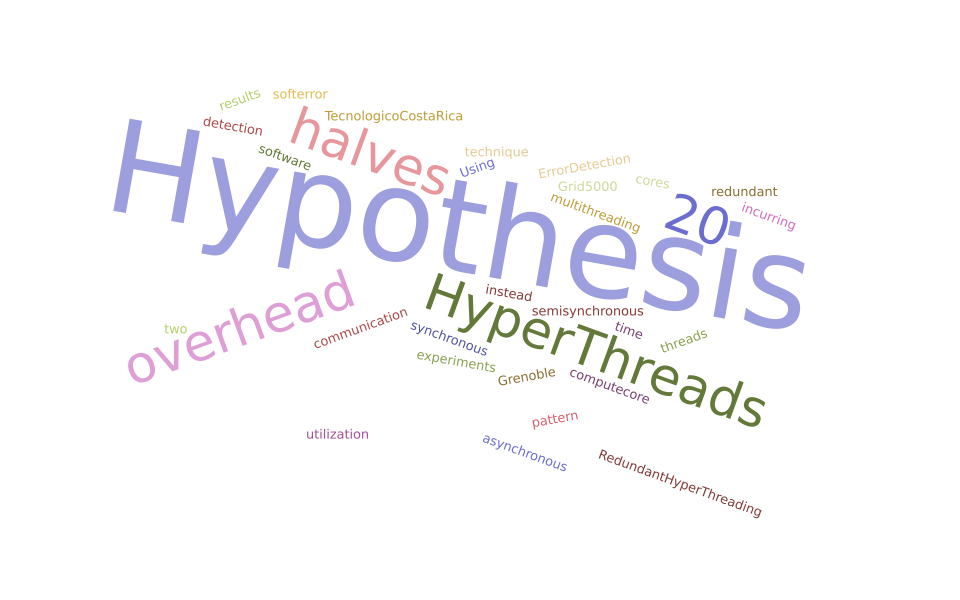
\includegraphics[scale=0.4]{WordCloudHypothesis.png} 
	%	\end{center}
	%\end{figure}
            
\end{frame}

\begin{frame}
	\frametitle{Proposed Solution - Specific Obj - Calendar 2018}
    
    \underline{Specific Objectives} 
    \begin{enumerate}
		\item Design the RHT exploiting Intel HT infrastructure.
		\item Implement the RHT in the C programming language. 
		\item Evaluate the performance RHT and compare to the same strategy with threads on different cores. 
	\end{enumerate} \pause

\underline{Deliverables Calendar 2018} 
\begin{center}
    \begin{tabular}{| l | l | l |} \hline
    	\textbf{Month} & \textbf{Activity} \\ \hline
    	February & Software installation on Grid 5000 machines.  \\ \hline
    	March & Specific Objective 1. \\ \hline
    	April & Specific Objective 2. \\ \hline
    	May & Specific Objective 3. \\ \hline 
        June & Final writing of thesis document. \\ \hline 
    \end{tabular}
\end{center}

\end{frame}

%\begin{frame}
%	\frametitle{Test Methodology}
%
%	\begin{columns}[c]
%	\column{2.3in}
%    	\begin{itemize}
%        	\item \onslide<1->{ \textit{Grid5000}, a large-scale testbed for experiment-driven research in computer science. Large amount of resources: 1000 nodes, 8000 cores. }
%        \end{itemize}
%    
%    \column{1.5in}
%    	\onslide<1->{
%    		\begin{figure}[H]
%    			\begin{center}
%        			
\includegraphics[scale=0.22]{TestPlan.png}
%         		\end{center}
%    		\end{figure}
%       }
%	\end{columns}
%
%    \begin{itemize}        
%        \item \onslide<2->{ Test HPC representative applications, part of the \textit{Mantevo} Project. }
%		\item \onslide<3->{ \textit{perf} counts hardware events such as instructions executed, cache misses suffered, or branches mispredicted. They form a basis for profiling applications. }
%     \end{itemize}
              
%\end{frame}

\section{Conclusions}
\begin{frame}
	\frametitle{Conclusions}
        
    \begin{itemize}
        \item Current multi-core chips are more susceptible to soft errors. 
        \item RMT is a soft error detection technique, with frequent inter-thread communication (performance bottleneck). 
        \item HT has not been properly investigated in RMT approaches. 
        \item Redundant Hyper-Threading technique will help mitigate the performance overhead. \pause
     \end{itemize}
     
     \definecolor{shadecolor}{rgb}{0.9,0.5,0.007}
    \begin{shaded}
    	\centerline{\textbf{Thanks! Questions? Comments?}}
    \end{shaded}
     
\end{frame}

	

\end{document}